\chapter{Activation Function}

Activation functions are needed in order to increase the complexity of the NN, without them it would just be a linear sandwich of linear functions (multiplying linear functions = linear function)


\section{Sigmoid}

\begin{figure}[!htb]
  \centering
  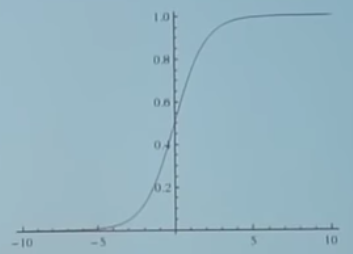
\includegraphics[width=0.3\textwidth]{Images/activation_f/1.png}
  \caption{Sigmoid }
\end{figure}
$\sigma (x) = \frac{1}{1+e^{-x}}$
\begin{itemize}
\item \textcolor{red}{Saturated neurons "kill" the gradient}
\item \textcolor{red}{No zero-centered output}
\item \textcolor{red}{exp() is computationaly expensive}
\end{itemize}


\section{Tanh}
\begin{figure}[!htb]
  \centering
  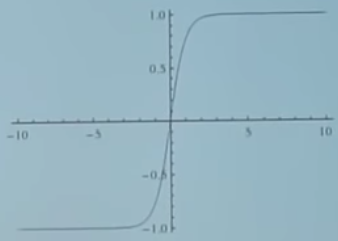
\includegraphics[width=0.3\textwidth]{Images/activation_f/2.png}
  \caption{Tanh }
\end{figure}
$\text{tanh} (x) = \frac{2}{e^{-2x}+1}-1$
\begin{itemize}
\item \textcolor{green}{Zero centered output}
\item \textcolor{red}{Saturated neurons "kill" the gradient}
\end{itemize}


\section{ReLU}
\begin{figure}[!htb]
  \centering
  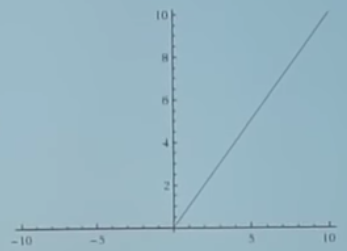
\includegraphics[width=0.3\textwidth]{Images/activation_f/3.png}
  \caption{ReLU }
\end{figure}
$f(x) = \max(0,x)$ If a neuron has $x < 0$ the ReLU kills it in backprop. The gradient will be 0 so that neuron will not backprop downwards and its weights will not be updated. Its like a boolean gate. The gradient in the case of $x=0$ is undefined (unlike case).

\begin{itemize}
\item \textcolor{green}{Does not saturate}
\item \textcolor{green}{Computationally efficient}
\item \textcolor{green}{Converges mch faster than sigmoid/tanh in practive ($~6x$)}

\item \textcolor{red}{Not zero centred output}
\item \textcolor{red}{If your unlucky a neuron may be never active because the initialization has put it outside the manifold.}
\item \textcolor{red}{When the learning rate is high is easy to kill a lot of neurons. Imagine the activation function as a threshold which is moving while training. If the learning rate is to high it may move out of the data manifold. In that case the neuron dies and will never be able to recover because will never update again.}
\end{itemize}

It is a good practice to initialize them with a slightly positive initial bias to avoid "dead neurons"

\section{Leaky ReLU}
\begin{figure}[h]
  \centering
  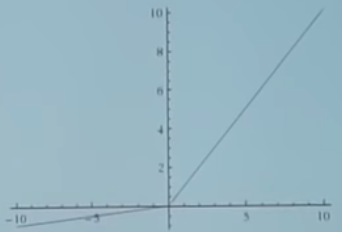
\includegraphics[width=0.3\textwidth]{Images/activation_f/5.png}
  \caption{Leaky ReLU}
\end{figure}
$f(x) = \max(\alpha x,x) = \left\{\begin{matrix}
\alpha x & \text{if}(x\leq 0)\\ 
x & \text{if}(x>  0)
\end{matrix}\right.$
where  $\alpha$ is a very small number $~0.01$ which can be a hyperparameter or learned through .

\begin{itemize}
\item \textcolor{green}{Does not saturate}
\item \textcolor{green}{Computationally efficient}
\item \textcolor{green}{Converges much faster than sigmoid/tanh in practice ($~6x$)}
\item \textcolor{green}{Does not die}

\item \textcolor{red}{Not zero centred output}
\item \textcolor{red}{Consistency of the benefits across tasks not clear}
\end{itemize}

\section{ELU - Exponential Linear Units}

\begin{figure}[!htb]
  \centering
  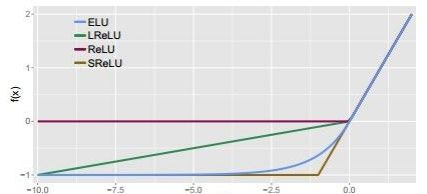
\includegraphics[width=0.5\textwidth]{Images/activation_f/6.png}
  \caption{ELU}
\end{figure}
$f(x) = \left\{\begin{matrix}
\alpha(e^x-1) & \text{if}(x\leq 0)\\ 
x & \text{if}(x>  0)
\end{matrix}\right.$
\begin{itemize}
\item \textcolor{green}{All benefits of ReLu}
\item \textcolor{green}{Does not die}
\item \textcolor{green}{Closer to zero mean outputs}

\item \textcolor{red}{exp() is computationally expensive}
\item \textcolor{red}{There is controversy if it actually trains better with this than with ReLU}
\end{itemize}

\section{Maxout}

\begin{figure}[!htb]
  \centering
  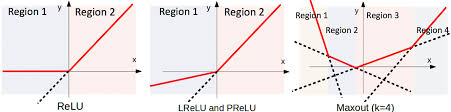
\includegraphics[width=0.6\textwidth]{Images/activation_f/7.jpg}
  \caption{Maxout}
\end{figure}
$f(x) = \max(w_1^Tx+b_1,w_2^Tx+b_2)$
\begin{itemize}
\item \textcolor{green}{Generalized ReLU and Leaky ReLU}
\item \textcolor{green}{Does not saturate}
\item \textcolor{green}{Does not die}
\item \textcolor{green}{Linear Regime}

\item \textcolor{red}{Doubles the number of parameters/neuros}
\end{itemize}

\section*{Conclusion}
\begin{itemize}
\item \textbf{Use ReLU} but be careful with your learning rates. So for example a 3-layer neural network will look like this: $f(x) = W_3 \text{max} (0,W_2 \text{max} (0, W_1x))$
\item Try out Leaky ReLU/Maxout/ELU
\item Try out tanh but don't expect much
\item Don't use sigmoid
\end{itemize}
